For the purposes of this work, we implemented several conversational, directed gaze behaviors on a virtual agent. These behaviors include: (1) body orientation shifts to reconfigure the F-formation, (2) gaze patterns to establish footing, and (3) gaze cues to indicate listening, addressing, and floor release.

\subsection{Reconfiguring the F-formation}

The current work considers multiparty interaction centered on a virtual agent, who could be serving in the role of an instructor, storyteller, customer service representative, or non-player character in a multiplayer game. When a user approaches the agent, the latter must turn to face the user and thus invite them to engage in an interaction, creating a so-called vis-a-vis arrangement~\cite{kendon1990conducting}. If one or more avatar-embodied users are already present in the interaction, the agent must reorient its body such that it distributes its attention among the users as evenly as possible, creating an approximately circular arrangement.

\begin{figure}
\centering
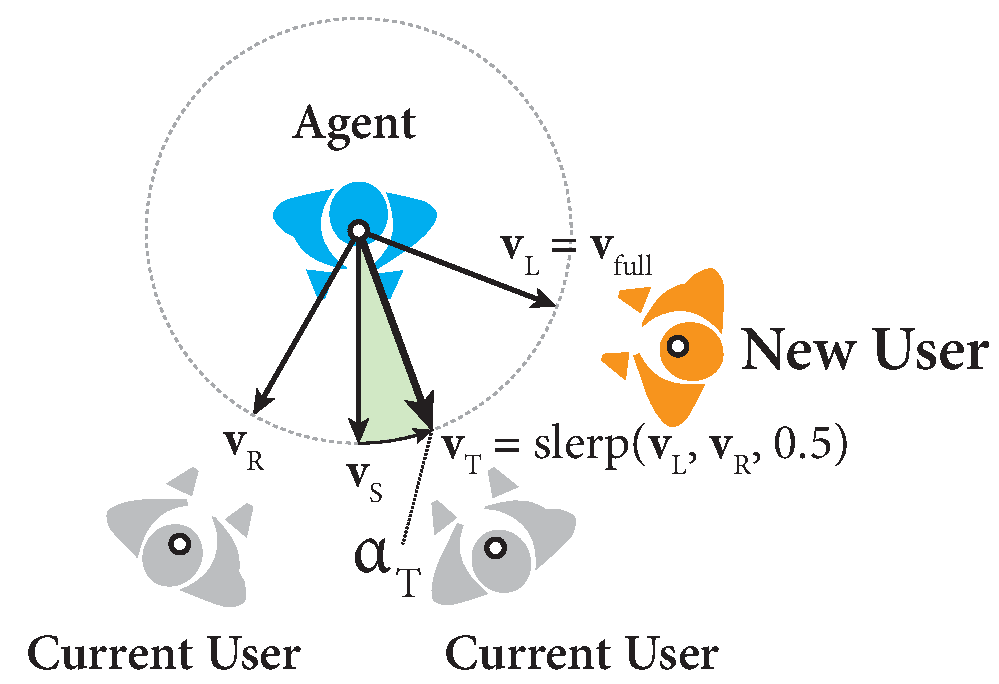
\includegraphics[width=0.9\textwidth]{conversationalrolegaze/Figures/FTorsoAlign.pdf}
\caption{Computing the torso alignment parameter $\alpha_T$ need for the agent to reconfigure the F-formation when a new user has joined the interaction.}
\label{fig:FTorsoAlign}
\end{figure}

To implement these behaviors, we use our gaze shift model (Chapter~\ref{cha:GazeShiftModel}) to execute the body orientation shifts. When the first user approaches the agent, the agent performs a gaze shift toward the user with the head, torso, and whole-body alignment parameters all set to 1 ($\alpha_H = alpha_T = alpha_B = 1$). This results in the agent facing the user head-on. If users are already present in the interaction, the agent must perform a gaze shift toward the new user that evenly distributes its body orientation among all the users. We set $\alpha_H = 1$ and $\alpha_B = 1$ as before, whereas $\alpha_T$ must be set such that the agent ends up oriented toward the midpoint between the leftmost and rightmost user. The procedure for computing $\alpha_T$ is as follows (Figure~\ref{fig:FTorsoAlign}). Let us define the following direction vectors:

\begin{enumerate}
\item $\mathbf{v}_S$ -- Current torso facing direction of the agent.
\item $\mathbf{v}_T$ -- Target torso facing direction of the agent.
\item $\mathbf{v}_\mathrm{full}$ -- Torso facing direction which would fully align the agent with the new user.
\item $\mathbf{v}_L$ -- Direction vector from the agent to the leftmost user.
\item $\mathbf{v}_R$ -- Direction vector from the agent to the rightmost user.
\end{enumerate}

All direction vectors are projected onto the horizontal plane. The agent must realign its body such that its torso facing direction ends up the following: $\mathbf{v}_T = \mathop{slerp}(\mathbf{v}_L, \mathbf{v}_R, 0.5)$. The torso alignment $\alpha_T$ needed to achieve that facing direction is:
%
\begin{align} \label{eq:FTorsoAlign}
\alpha_T = \frac{\angle(\mathbf{v}_S, \mathbf{v}_T)}{\angle(\mathbf{v}_S, \mathbf{v}_\mathrm{full})}
\end{align}
%

\subsection{Gaze Patterns for Footing}

~\citet{mutlu2012conversational} report probability distributions of participants' gaze among each other and the environment. We implement the agent's gaze patterns based on their data. In our implementation, participants distribute their gaze roughly equally among each other and only occasionally glance at bystanders---individuals who are listening in on the interaction without being a part of it. They alternate between making eye contact, looking at the other person's torso, or looking at a spot in the environment. Frequent gaze aversions toward the torso and the environment serve the purpose of intimacy regulation---staring into another person's eyes for long periods of time is known to cause discomfort~\citep{argyle1976gaze}.

\begin{table}
\centering
\def\arraystretch{1.5}
\begin{tabular}{|l|l|r|}
\hline
\textbf{Gaze Target} & \textbf{Footing Configuration} & \textbf{Gaze Probability} \\
\hline
\multirow{2}{*}{Addressee \emph{face}} & 1 addressee & 26\% \\
& 2+ addressees & 52\% / \# addressees \\
\hdashline
\multirow{2}{*}{Addressee \emph{torso}} & 1 addressee & 48\% \\
& 2+ addressees & 16\% / \# addressees \\
\hdashline
\multirow{2}{*}{Bystander \emph{face}} & 1 bystander & 5\% \\
& 2+ bystanders & 8\% / \# bystanders \\
\hdashline
\multirow{2}{*}{Bystander \emph{torso}} & 1 bystander & 3\% \\
& 2+ bystanders & 5\% / \# bystanders \\
\hdashline
\multirow{6}{*}{Environment} & 1 addressee, no bystanders & 26\% \\
& 1 addressee, 1 bystander & 18\% \\
& 1 addressee, 2+ bystanders & 13\% \\
& 2+ addressees, no bystanders & 32\% \\
& 2+ addressees, 1 bystander & 26\% \\
& 2+ addressees, 2+ bystanders & 19\% \\
\hline
\end{tabular}
\caption{Spatial distributions of the agent's gaze while speaking or waiting for user speech, expressed as probability of looking at a target in the given configuration of conversational roles.}
\label{tab:GazeFootingSpatial}
\end{table}

\begin{table}
\centering
\def\arraystretch{1.5}
\begin{tabular}{|l|l|r|}
\hline
\textbf{Gaze Target} & \textbf{Footing Configuration} & \textbf{Fixation Length} \\
\hline
\multirow{3}{*}{Addressee \emph{face}} & 1 addressee, no bystanders & $\mathop{Gamma}(k = 1.65, \Phi = 0.56)}$ \\
& 1 addressee, 1 bystander & $\mathop{Gamma}(k = 0.74, \Phi = 1.55}$ \\
& 2+ addressee & $\mathop{Gamma}(k = 1.48, \Phi = 1.10}$ \\
\hdashline
\multirow{3}{*}{Addressee \emph{torso}} & 1 addressee, no bystanders & $\mathop{Gamma}(k = 1.92, \Phi = 0.84}$ \\
& 1 addressee, 1 bystander & $\mathop{Gamma}(k = 1.72, \Phi = 1.20}$ \\
& 2+ addressee & $\mathop{Gamma}(k = 1.92, \Phi = 0.52}$ \\
\hdashline
Bystander \emph{face} & 1+ bystanders & $\mathop{Gamma}(k = 2.19, \Phi = 0.44}$ \\
\hdashline
Bystander \emph{torso} & 1+ bystanders & $\mathop{Gamma}(k = 1.76, \Phi = 0.57}$ \\
\hdashline
\multirow{3}{*}{Environment} & 1 addressee, no bystanders & $\mathop{Gamma}(k = 0.90, \Phi = 1.14}$ \\
& 1 addressee, 1 bystander & $\mathop{Gamma}(k = 1.84, \Phi = 0.59}$ \\
& 2+ addressee & $\mathop{Gamma}(k = 2.23, \Phi = 0.41}$ \\
\hline
\end{tabular}
\caption{Agent's gaze fixation lengths (in seconds), expressed as gamma distributions specifying the length of fixation of a target in the given configuration of conversational roles.}
\label{tab:GazeFootingFixationLengths}
\end{table}

Table~\ref{tab:GazeFootingSpatial} specifies the probabilities of the agent gazing at a particular target. Possible targets include: addresssees' and bystanders' faces and torso, and randomly chosen locations in the environment. These probabilities change depending on the number of participants and their footing. As the agent speaks or waits for a user to take the floor, the targets of its gaze shifts are selected by drawing from these distributions. Gaze fixation durations are determined by drawing from the gamma distributions given in Table~\ref{tab:GazeFootingFixationLengths}. Consider an example: the agent is speaking with two addressees (A and B), with two bystanders present. When the time comes to shift the agent's gaze, we use the distributions in Table~\ref{tab:GazeFootingSpatial} to determine the target of the gaze shift. The probability of looking at addressee A's face is $52\% / 2 = 26\%$ (Table~\ref{tab:GazeFootingSpatial}, second row); let us assume this is the target we have chosen by randomly drawing from the distribution. Next, we need to determine how long to fixate the gaze on addressee A's face. We generate the fixation length by drawing from the distribution $\mathop{Gamma}(k = 1.48, \Phi = 1.10$ (Table~\ref{tab:GazeFootingFixationLengths}, third row).

The agent uses the gaze patterns for footing while it is speaking or while waiting for a user to speak (i.e., after releasing the floor.) It also uses several other patterns that override those. Firstly, when beginning a speech utterance, the agent always looks into the face of the addressee; if there are multiple addressees, the agent randomly chooses between them. Secondly, at the end of the utterance, the agent always looks back at the addressee's face as it released the floor to them. Thirdly, while a user is speaking, the agent is always looking at their face, with frequent gaze aversions generated using the Eyes Alive model~\citep{lee2002eyes}.